

\begin{center}
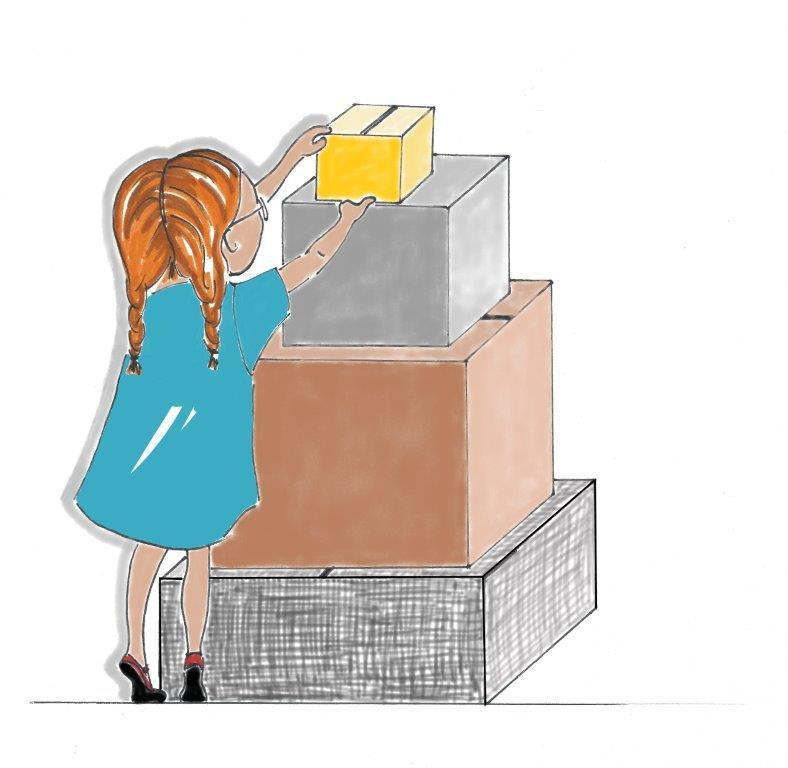
\includegraphics[width=0.6\textwidth]{content/3/chapter4/images/11.png}\\
Cippi在准备包裹
\end{center}

模块是C++20的四大特性之一,模块的功能有很多:编译时间短,隔离宏,取消头文件,避免工作区。在介绍模块的优点之前,先来了解一下模块。

\subsubsubsection{4.2.1\hspace{0.2cm}为什么需要模块?}

从一个简单的可执行文件开始:

\begin{lstlisting}[style=styleCXX]
// helloWorld.cpp

#include <iostream>

int main() {
	std::cout << "Hello World" << '\n';
}
\end{lstlisting}

使用\href{http://gcc.gnu.org/}{GCC}可将helloWorld.cpp编译成一个可执行的helloWorld,可执行文件的大小是文本文件的130倍。

\begin{center}
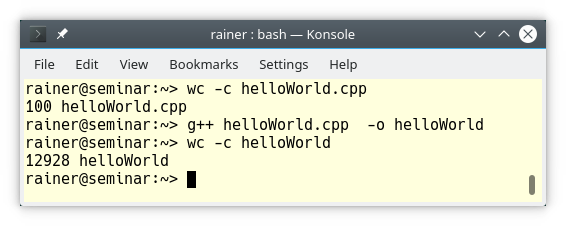
\includegraphics[width=0.8\textwidth]{content/3/chapter4/images/12.png}\\
目标文件的大小
\end{center}

截图中的数字100和12928代表字节数。现在,我们再对底层发生的事情进行一下了解。

\hspace*{\fill} \\ %插入空行
\noindent
\textbf{4.2.1.1\hspace{0.2cm}传统的构建过程}

构建过程包括三个步骤:预处理、编译和链接。

\hspace*{\fill} \\ %插入空行
\noindent
\textbf{4.2.1.1.1\hspace{0.2cm}预处理}

预处理器以\#include和\#define的方式处理指令。预处理器用相应的头文件替换\#include指令,并替换宏(\#define)。因为诸如\#if,\#else,\#elif,\#ifdef,\#ifndef和\#endif等指令,源代码的一部分可以包含或排除。

这个简单的文本替换过程(宏展开)可以通过在GCC/Clang上使用编译器标志-E,或在Windows上使用/E,就可以进行查看了。

\begin{center}
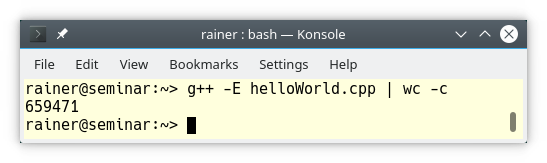
\includegraphics[width=0.8\textwidth]{content/3/chapter4/images/13.png}\\
预处理器的输出
\end{center}

哇! !预处理步骤的输出超过50万个字节。我不想责怪GCC,因为其他编译器也有同样的情况。预处理器的输出则是编译器的输入。

预处理步骤的结果就是翻译单元。

\hspace*{\fill} \\ %插入空行
\noindent
\textbf{4.2.1.1.2\hspace{0.2cm}编译}

编译器在预处理器的输出上执行编译,解析C++源代码,并将其转换为汇编代码。生成的文件称为目标文件,包含二进制形式的编译代码。目标文件可以引用没有定义的符号,也可以放在存档文件中以供后续重用。这些存档文件称为静态库。

编译器生成的对象文件则是链接器的输入。

\hspace*{\fill} \\ %插入空行
\noindent
\textbf{4.2.1.1.3\hspace{0.2cm}连接}

链接器的输出可以是可执行文件、静态库或动态库。链接器的工作是解析对未定义符号的引用,符号在目标文件或库中定义。这个阶段常见的错误是符号没有定义或者定义了不止一次。

这个由三个步骤组成的构建过程继承自C。若只有一个翻译单元,就能很好地工作。但若有不止一个翻译单元,就会出现很多问题。

\hspace*{\fill} \\ %插入空行
\noindent
\textbf{4.2.1.2\hspace{0.2cm}构建中的问题}

下面是经典构建过程中缺陷的不完整列表,这些缺陷可以通过模块来解决。

\hspace*{\fill} \\ %插入空行
\noindent
\textbf{4.2.1.2.1\hspace{0.2cm}重复替换}

预处理器用相应的头文件替换\#include指令。修改一下helloWorld.cpp程序,重构了程序并添加了两个源文件hello.cpp和world.cpp。源文件hello.cpp提供了hello函数,源文件world.cpp提供了world函数。

两个源文件都包含相应的头文件。重构意味着具有与前面的程序helloWorld.cpp相同的外部行为,但内部结构进行了改进。以下是新文件:

\begin{itemize}
\item 
hello.cpp和hello.h

\begin{lstlisting}[style=styleCXX]
// hello.cpp

#include "hello.h"

void hello() {
	std::cout << "hello ";
}
\end{lstlisting}

\begin{lstlisting}[style=styleCXX]
// hello.h

#include <iostream>

void hello();
\end{lstlisting}

\item 
world.cpp和world.h

\begin{lstlisting}[style=styleCXX]
// world.cpp

#include "world.h"

void world() {
	std::cout << "world";
}
\end{lstlisting}

\begin{lstlisting}[style=styleCXX]
// world.h

#include <iostream>

void world();
\end{lstlisting}

\item 
helloWorld2.cpp

\begin{lstlisting}[style=styleCXX]
// helloWorld2.cpp

#include <iostream>

#include "hello.h"
#include "world.h"

int main() {
	
	hello();
	world();
	std::cout << '\n';
}
\end{lstlisting}


\end{itemize}

构建和执行如预期的一样:

\begin{center}
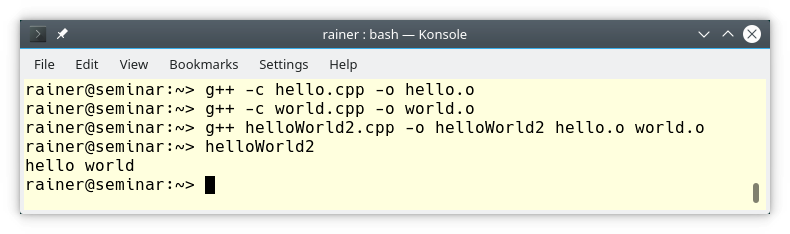
\includegraphics[width=0.8\textwidth]{content/3/chapter4/images/14.png}\\
编译一个简单程序
\end{center}

问题是这样的。预处理器运行在每个源文件上,所以头文件<iostream>总共包含了三次。因此,每个源文件均多了50多万行代码。

\begin{center}
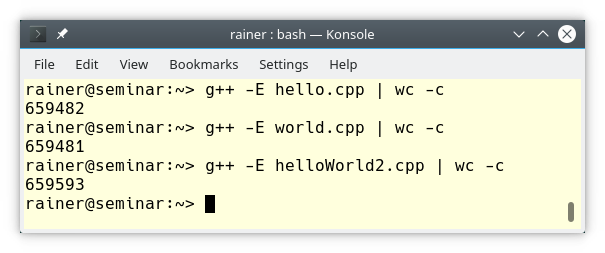
\includegraphics[width=0.8\textwidth]{content/3/chapter4/images/15.png}\\
预处理源文件的大小
\end{center}

这是对编译时间的浪费。与头文件不同,模块只导入一次,所以不会有什么开销。

\hspace*{\fill} \\ %插入空行
\noindent
\textbf{4.2.1.2.2\hspace{0.2cm}隔离预处理宏}

若C++社区有一个共识的话,那就是:应该去掉预处理器宏。为什么?使用宏只是简单的文本替换,不包括任何C++语义。当然,这有许多负面后果:例如,这可能取决于包含宏的顺序,或者宏可能与应用程序中已经定义的宏或名称冲突。

假设有两个头文件webcolors.h和productininfo.h。

\hspace*{\fill} \\ %插入空行
\noindent
\textbf{先定义一个宏RED}
\begin{lstlisting}[style=styleCXX]
// webcolors.h
#define RED 0xFF0000
\end{lstlisting}

\noindent
\textbf{再定义一个宏RED}
\begin{lstlisting}[style=styleCXX]
// productinfo.h
#define RED 0
\end{lstlisting}

当源文件client.cpp包含两个头文件时,宏RED的值取决于所包含头文件的顺序。这种依赖关系非常容易出错。

模块则没有导入顺序的问题。

\hspace*{\fill} \\ %插入空行
\noindent
\textbf{4.2.1.2.3\hspace{0.2cm}隔离宏}

ODR代表单一定义规则,对于函数:

\begin{itemize}
\item 
函数在任何翻译单元中不能有多于一个的定义。

\item 
函数在程序中不能有多个定义。
\end{itemize}

可以在多个翻译单元中定义具有外部链接的内联函数,而宏必须满足每个定义的要求。

当链接违背单一定义规则的程序时,链接器会怎么样呢?下面的代码示例有两个头文件,header.h和header2.h。主程序包含头文件header.h两次,由于包含了func的两个定义,因此违背了单一定义规则。

\hspace*{\fill} \\ %插入空行
\noindent
\textbf{函数func的定义}
\begin{lstlisting}[style=styleCXX]
// header.h
void func() {}
\end{lstlisting}

\noindent
\textbf{将函数定义间接包含到func中}
\begin{lstlisting}[style=styleCXX]
// header2.h
#include "header.h"
\end{lstlisting}

\noindent
\textbf{双重定义的函数func}
\begin{lstlisting}[style=styleCXX]
// main.cpp

#include "header.h"
#include "header2.h"

int main() {}
\end{lstlisting}

链接器会说,func有多个定义:

\begin{center}
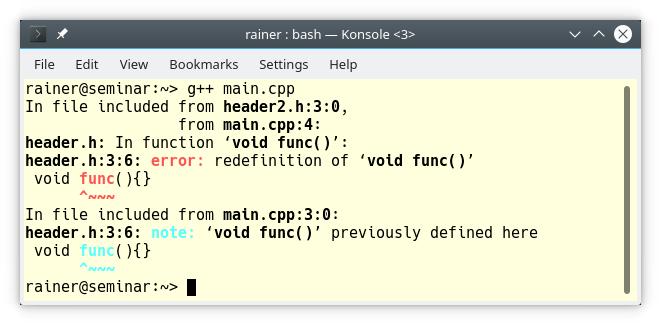
\includegraphics[width=0.8\textwidth]{content/3/chapter4/images/16.png}\\
违背了单一定义规则
\end{center}

我们已经习惯了一些丑陋的方法,比如:在头文件周围加一个包含守卫。在头文件header.h中添加包含守卫FUNC\_H可以解决这个问题。

\hspace*{\fill} \\ %插入空行
\noindent
\textbf{使用包含守卫来解决ODR问题}
\begin{lstlisting}[style=styleCXX]
// header.h

#ifndef FUNC_H
#define FUNC_H

void func(){}

#endif
\end{lstlisting}

对于模块,不太可能出现重复符号。

那么,现在我就来聊聊模块的优势。

\subsubsubsection{4.2.2\hspace{0.2cm}优势}

下面以简洁的形式介绍模块的优势:

\begin{itemize}
\item 
模块只导入一次,编译开销很小。

\item 
导入模块没有顺序的区别。

\item 
模块不可能出现重复符号。

\item 
模块能够表达代码的逻辑结构。可以显式地指定应导出或不应导出的名称,还可以将几个模块捆绑到一个更大的模块中,并将它们作为逻辑包提供出去。

\item 
不需要再将源代码分离为接口和实现部分。
\end{itemize}

\begin{tcolorbox}[breakable,enhanced jigsaw,colback=blue!5!white,colframe=blue!75!black,title={常规类型}]

C++中的模块可能比你想象的要更加古老。简短的历史回顾应该能让你了解,把如此有价值的东西纳入C++标准需要多长时间。

\hspace*{\fill} \\ %插入空行
2004年,Daveed Vandevoorde写了一份提案\href{http://www.open-std.org/jtc1/sc22/wg21/docs/papers/2004/n1736.pdf}{N1736.pdf},第一次描述了模块的思想。不过,直到2012年才成立了专门的研究小组(SG2,模块)。2017年,Clang 5.0和MSVC 19.1提供了第一个实现。2018年,模块TS(技术规范)确定。大约在同一时间,Google针对模块提出了ATOM(Another Take On Modules)提案(\href{http://www.open-std.org/jtc1/sc22/wg21/docs/papers/2018/p0947r1.html}{P0947})。2019年,模块TS和ATOM提案合并到C++20委员会草案中(\href{https://github.com/cplusplus/draft/releases/tag/n4842}{N4842})。
\end{tcolorbox}

\subsubsubsection{4.2.3\hspace{0.2cm}举个例子}

本节的目的很简单:介绍模块。模块的更高级特性将在后面几节中介绍。

先从一个简单的数学模块开始吧。

\hspace*{\fill} \\ %插入空行
\noindent
\textbf{简单的math模块}
\begin{lstlisting}[style=styleCXX]
// math.ixx

export module math;

export int add(int fir, int sec){
	return fir + sec;
}
\end{lstlisting}

表达式导出模块math是模块声明。通过将export放在函数add的定义之前,将add导出。

\hspace*{\fill} \\ %插入空行
\noindent
\textbf{使用math模块}
\begin{lstlisting}[style=styleCXX]
// client.cpp

import math;

int main() {
	add(2000, 20);
}
\end{lstlisting}

import math导入math模块,并使模块中导出的名称对client.cpp可见。

\hspace*{\fill} \\ %插入空行
\noindent
\textbf{4.2.3.1\hspace{0.2cm}模块的声明文件}

是否注意到模块的奇怪名称:math.ixx。

\begin{itemize}
\item 
Microsoft编译器使用扩展名ixx,后缀ixx代表模块接口源。

\item 
Clang编译器最初使用扩展cppm,后缀中的m可能代表模块。这个约定在Clang的新版本中更改为cpp扩展(不使用后缀的方式来区分模块)。

\item 
GCC编译器则不使用特殊的扩展。
\end{itemize}

全局模块用于组合模块接口,以关键字module开始,以模块声明结束。全局模块可以出现在使用预处理器指令(如\#include)的地方,以便模块接口可以编译。全局模块片段中的代码,不会由模块接口导出。

math模块的第二个版本支持add和getProduct两个函数。

\hspace*{\fill} \\ %插入空行
\noindent
\textbf{全局模块的定义}
\begin{lstlisting}[style=styleCXX]
// math1.ixx

module;

#include <numeric>
#include <vector>

export module math;

export int add(int fir, int sec){
	return fir + sec;
}

export int getProduct(const std::vector<int>& vec) {
	return std::accumulate(vec.begin(), vec.end(), 1, std::multiplies<int>());
}
\end{lstlisting}

我在全局模块(第3行)和模块声明(第8行)间包含了必要的头文件。

\hspace*{\fill} \\ %插入空行
\noindent
\textbf{使用改进的math模块}
\begin{lstlisting}[style=styleCXX]
// client1.cpp

#include <iostream>
#include <vector>

import math;

int main() {
	
	std::cout << '\n';
	
	std::cout << "add(2000, 20): " << add(2000, 20) << '\n';
	
	std::vector<int> myVec{1, 2, 3, 4, 5, 6, 7, 8, 9, 10};
	
	std::cout << "getProduct(myVec): " << getProduct(myVec) << '\n';
	
	std::cout << '\n';
}
\end{lstlisting}

客户端导入math模块,并使用其功能:

\begin{center}
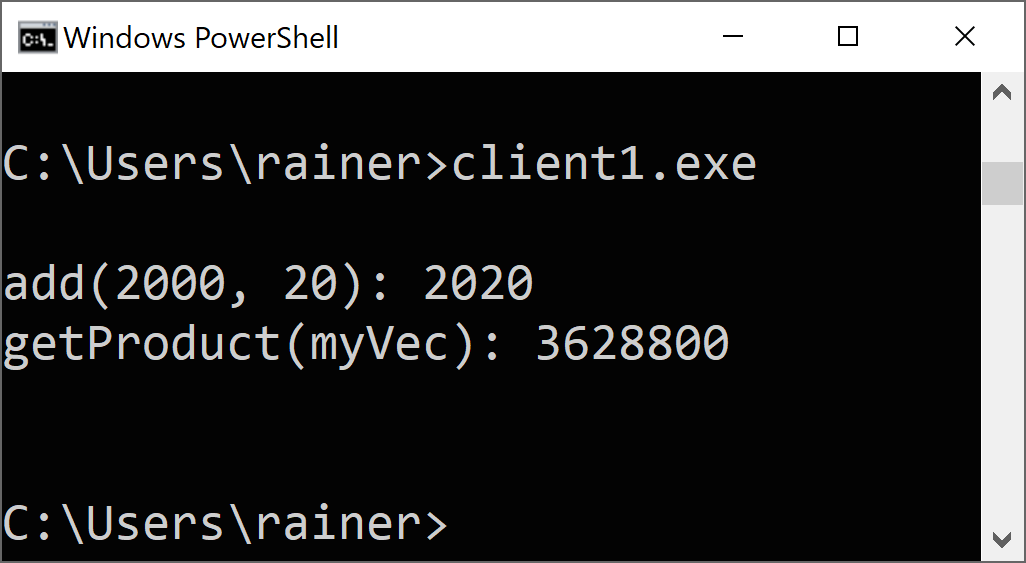
\includegraphics[width=0.5\textwidth]{content/3/chapter4/images/17.png}\\
执行程序client1.exe
\end{center}

现在,再了解一下细节。

\subsubsubsection{4.2.4\hspace{0.2cm}编译和使用}

编译math模块。若客户端程序client.cpp使用ixx,则必须使用最新的Clang、GCC或Microsoft编译器。

模块的编译还是具有挑战性,我将用Microsoft编译器和Clang编译器作为示例来演示模块的编译。

\hspace*{\fill} \\ %插入空行
\noindent
\textbf{4.2.4.1\hspace{0.2cm}Microsoft Visual编译器}

首先,我使用cl.exe 19.25.28614(x64)编译器。

\begin{center}
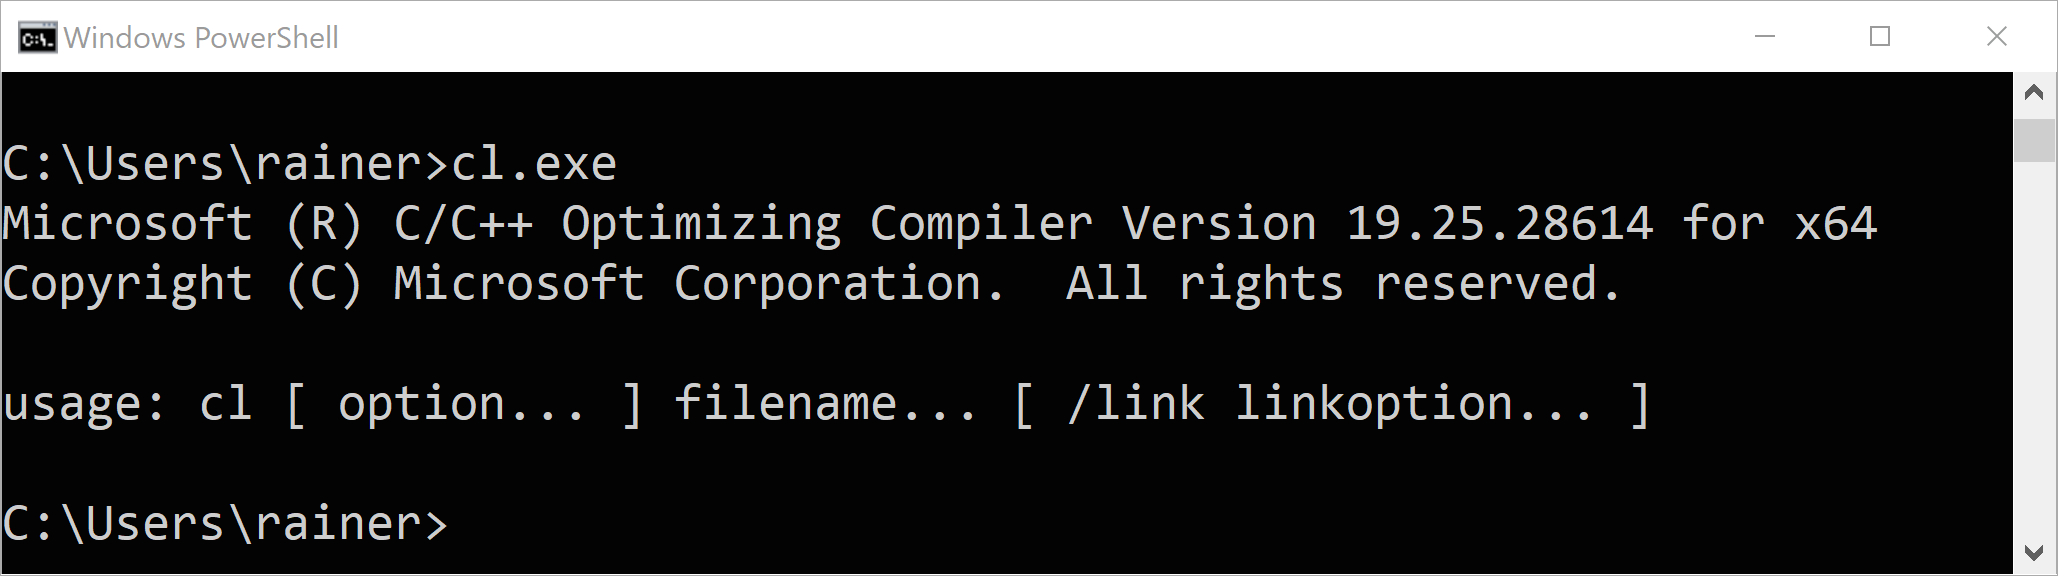
\includegraphics[width=0.8\textwidth]{content/3/chapter4/images/18.png}\\
Microsoft的编译器
\end{center}

这些是使用Microsoft编译器编译和使用模块的步骤,我只展示了最短的命令行示例。此外,对于旧的微软编译器,必须使用/std:cpplatest编译标志。

\hspace*{\fill} \\ %插入空行
\noindent
\textbf{使用Microsoft编译器构建可执行文件}
\begin{tcblisting}{commandshell={}}
cl.exe /std:c++latest /c math.ixx
cl.exe /std:c++latest client.cpp math.obj
\end{tcblisting}

\begin{itemize}
\item 
第1行创建一个目标文件math.obj和一个IFC文件math.ifc。IFC文件包含模块接口的元数据描述。IFC的二进制格式是模仿Gabriel Dos Reis和Bjarne Stroustrup(2004/2005)的\href{https://www.stroustrup.com/gdr-bs-macis09.pdf}{内部程序表示}。

\item 
第2行创建可执行文件client.exe。若第一步没有隐式使用math.ifc文件,则链接器无法找到模块。
\end{itemize}

这里,就不展示程序执行的输出了。

\hspace*{\fill} \\ %插入空行
\noindent
\textbf{4.2.4.2\hspace{0.2cm}Clang编译器}

在Linux上,我使用Clang 10.0.0编译器。

\begin{center}
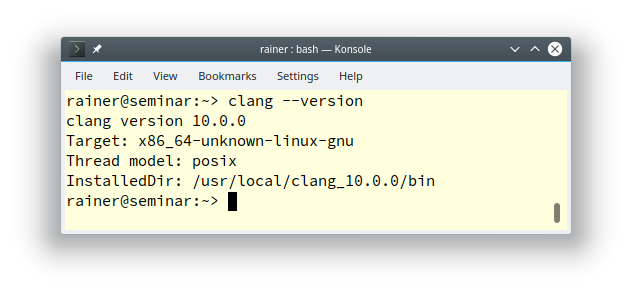
\includegraphics[width=0.8\textwidth]{content/3/chapter4/images/19.png}\\
Clang 10.0.0编译器
\end{center}

使用clang编译器,模块声明文件就是一个cpp文件,必须将math.ixx重命名为math.cpp。

\begin{lstlisting}[style=styleCXX]
// math.cpp

export module math;

export int add(int fir, int sec){
	return fir + sec;
}
\end{lstlisting}

客户端文件client.cpp没有改变,这是创建可执行文件的必要步骤。

\hspace*{\fill} \\ %插入空行
\noindent
\textbf{使用Clang编译器构建可执行文件}
\begin{tcblisting}{commandshell={}}
clang++ -std=c++20 -c math.cpp -Xclang -emit-module-interface -o math.pcm

clang++ -std=c++20 -fprebuilt-module-path=. client.cpp math.pcm -o client.exe
\end{tcblisting}

\begin{itemize}
\item 
第1行创建模块math.pcm,后缀pcm代表预编译模块。标志-std=c++2a指定C++20标准的工作草案,-stdlib=libc++指定使用的C++标准库。标记组合-Xclang -emit-module-interface是创建预编译模块所需的标志。

\item 
第4行创建可执行程序,使用模块math.pcm,并用-fprebuilt-module-path标志指定模块的路径。
\end{itemize}

\hspace*{\fill} \\ %插入空行
\noindent
\textbf{4.2.4.3\hspace{0.2cm}使用过的编译器}

我在这本书中使用的是Microsoft的cl.exe。Microsoft目前(2020年底)\href{https://en.cppreference.com/w/cpp/compiler_support}{对模块的最佳支持}的情况。Microsoft博客提供了两个很好的模块介绍:\href{https://docs.microsoft.com/en-us/cpp/cpp/modules-cpp?view=msvc-160&viewFallbackFrom=vs-2019}{概述C++模块}和\href{https://devblogs.microsoft.com/cppblog/c-modules-conformance-improvements-with-msvc-in-visual-studio-2019-16-5/}{C++模块的一致性改进与MSVC在Visual Studio 2019 16.5}。Clang和GCC都没有提供类似的介绍,因此在这些编译器中使用模块也非常困难。

\subsubsubsection{4.2.5\hspace{0.2cm}导出}

有三种方法可以导出模块接口单元中的名称。

\hspace*{\fill} \\ %插入空行
\noindent
\textbf{4.2.5.1\hspace{0.2cm}导出说明符}

可以显式地导出每个名称。

\begin{lstlisting}[style=styleCXX]
export module math;
export int mult(int fir, int sec);
export void doTheMath();
\end{lstlisting}

\hspace*{\fill} \\ %插入空行
\noindent
\textbf{4.2.5.2\hspace{0.2cm}导出组}

导出组会导出所有名称。

\begin{lstlisting}[style=styleCXX]
export module math;
export {
	int mult(int fir, int sec);
	void doTheMath();
}
\end{lstlisting}

\hspace*{\fill} \\ %插入空行
\noindent
\textbf{4.2.5.3\hspace{0.2cm}导出命名空间}

可以使用导出的命名空间,代替导出组。

\begin{lstlisting}[style=styleCXX]
export module math;
export namespace math {
	int mult(int fir, int sec);
	void doTheMath();
}
\end{lstlisting}

当客户端使用来自导出的命名空间时,必须限定这些名称。

只有没有内部链接的名称才可以导出。

\subsubsubsection{4.2.6\hspace{0.2cm}构造模块结构的指南}

来了解一下构造模块的指导方针。

\begin{lstlisting}[style=styleCXX]
module; // global module fragment
#include <headers for libraries not modularized so far>
export module math; // module declaration; starts the module purview
import <importing of other modules>
<non-exported declarations> // names only visibile inside the module
export namespace math {
	<exported declarations> // exported names
}
\end{lstlisting}

这个指导原则有一个目的:提供简化的模块结构,以及将要书写的内容。那么,这个模块结构有什么新东西呢?

\begin{itemize}
\item 
可选以关键字module开头的全局模块,之后和模块声明之前的位置,是包含头文件的正确位置。

\item 
模块声明导出模块math启动模块权限,该权限在翻译单元的末尾结束。

\item 
可以在模块权限的开始导入模块。导入的模块具有模块链接,在模块外部不可见。这一点也适用于非导出声明。
\end{itemize}
 
我将导出的名称放在命名空间math中,该名称与模块名称相同。
 
模块只有声明的名称。现在,一起来了解一下接口和模块的实现分离。

\subsubsubsection{4.2.7\hspace{0.2cm}模块接口单元和模块实现单元}

当模块变大时,应该将其组织成一个模块接口单元和一个或多个模块实现单元。按照前面提到的构造模块的指导原则重构math模块。

\hspace*{\fill} \\ %插入空行
\noindent
\textbf{4.2.7.1\hspace{0.2cm}模块接口单元}

\begin{lstlisting}[style=styleCXX]
// mathInterfaceUnit.ixx

module;

#include <vector>

export module math;

export namespace math {

	int add(int fir, int sec);
	
	int getProduct(const std::vector<int>& vec);

}
\end{lstlisting}

\begin{itemize}
\item 
模块接口单元包含导出模块声明:export module math(第7行)。

\item 
导出add和getProduct(第11和13行)。

\item 
一个模块只能有一个模块接口单元。
\end{itemize}

\hspace*{\fill} \\ %插入空行
\noindent
\textbf{4.2.7.2\hspace{0.2cm}模块的实现单元}

\begin{lstlisting}[style=styleCXX]
// mathImplementationUnit.cpp

module math;

#include <numeric>

namespace math {

	int add(int fir, int sec) {
		return fir + sec;
	}
	
	int getProduct(const std::vector<int>& vec) {
		return std::accumulate(vec.begin(), vec.end(), 1, std::multiplies<int>());
	}
}
\end{lstlisting}

\begin{itemize}
\item 
模块实现单元包含非导出模块声明:module math;(第3行)。

\item 
一个模块可以有多个模块实现单元。
\end{itemize}

\hspace*{\fill} \\ %插入空行
\noindent
\textbf{4.2.7.3\hspace{0.2cm}主程序}

\begin{lstlisting}[style=styleCXX]
// client3.cpp

#include <iostream>
#include <vector>

import math;

int main() {

	std::cout << '\n';
	
	std::cout << "math::add(2000, 20): " << math::add(2000, 20) << '\n';
	
	std::vector<int> myVec{1, 2, 3, 4, 5, 6, 7, 8, 9, 10};
	
	std::cout << "math::getProduct(myVec): " << math::getProduct(myVec) << '\n';
	
	std::cout << '\n';

}
\end{lstlisting}

从用户的角度来看,除了导入模块math(第6行),还需要添加命名空间math。

解释依赖于编译器,我把它们放在一个单独的提示框中。若各位想尝试一下,可以参考这些信息。


\begin{tcolorbox}[breakable,enhanced jigsaw,colback=blue!5!white,colframe=blue!75!black,title={使用Microsoft编译器构建可执行文件}]
	
手动构建可执行文件包括以下几个步骤。

\hspace*{\fill} \\ %插入空行
\noindent
\textbf{用模块接口单元和模块实现单元构建模块}
{\footnotesize
\begin{tcblisting}{commandshell={}}
cl.exe /c /experimental:module mathInterfaceUnit.ixx /EHsc
cl.exe /c /experimental:module mathImplementationUnit.cpp /EHsc
cl.exe /c /experimental:module client3.cpp /EHsc
cl.exe client3.obj mathInterfaceUnit.obj mathImplementationUnit.obj
\end{tcblisting}
}

\begin{itemize}
\item 
第1行:创建了对象文件mathInterfaceUnit.obj和模块接口文件math.ifc。

\item 
第2行:创建了对象文件mathImplementationUnit.obj。

\item 
第3行:创建对象文件client3.obj。

\item 
第4行:创建可执行文件client3.exe。
\end{itemize}

对于Microsoft编译器,必须指定异常处理模型(/EHsc),并启用模块支持:/experimental:module。

最后,是程序的输出:

\begin{center}
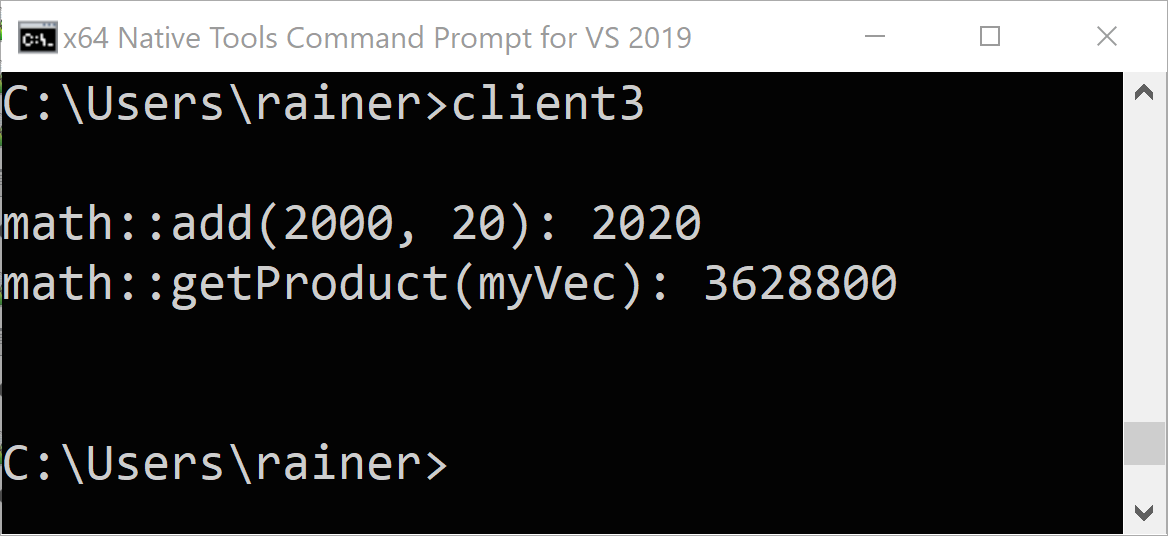
\includegraphics[width=0.6\textwidth]{content/3/chapter4/images/20.png}\\
执行程序client2.exe
\end{center}
\end{tcolorbox}

\subsubsubsection{4.2.8\hspace{0.2cm}子模块和模块分区}

当模块变大时,可以将其功能划分为可管理的组件。C++20模块提供了两种方法:子模块和分区。

\hspace*{\fill} \\ %插入空行
\noindent
\textbf{4.2.8.1\hspace{0.2cm}子模块}

模块可以导入模块,然后重新导出它们。

下面的例子中,math模块导入了子模块math.math1和math.math2。

\begin{lstlisting}[style=styleCXX]
// mathModule.ixx
export module math;
export import math.math1;
export import math.math2;
\end{lstlisting}

表达式export import math.math1将math.math1导入math模块,并将其作为math模块的一部分重新导出。

完整起见,下面是完整的math.math1和math.math2。我使用单独的代码段,将math模块与其子模块分开。实际开发中,代码没必要分开。

\hspace*{\fill} \\ %插入空行
\noindent
\textbf{子模块math.math1}
\begin{lstlisting}[style=styleCXX]
// mathModule1.ixx
export module math.math1;
export int add(int fir, int sec) {
	return fir + sec;
}
\end{lstlisting}

\noindent
\textbf{子模块math.math2}
\begin{lstlisting}[style=styleCXX]
// mathModule2.ixx
export module math.math2;
export {
	int mul(int fir, int sec) {
		return fir * sec;
	}
}
\end{lstlisting}

仔细观察会发现,math模块中的export语句相较之前有所不同。math.math1使用导出说明符,而math.math2则使用导出组或导出块。

从使用者的角度来看,使用math模块非常简单。

\hspace*{\fill} \\ %插入空行
\noindent
\textbf{主程序}
\begin{lstlisting}[style=styleCXX]
// mathModuleClient.cpp
#include <iostream>
import math;
int main() {
	std::cout << '\n';
	std::cout << "add(3, 4): " << add(3, 4) << '\n';
	std::cout << "mul(3, 4): " << mul(3, 4) << '\n';
}
\end{lstlisting}

编译和执行程序可以得到预期输出。

\begin{center}
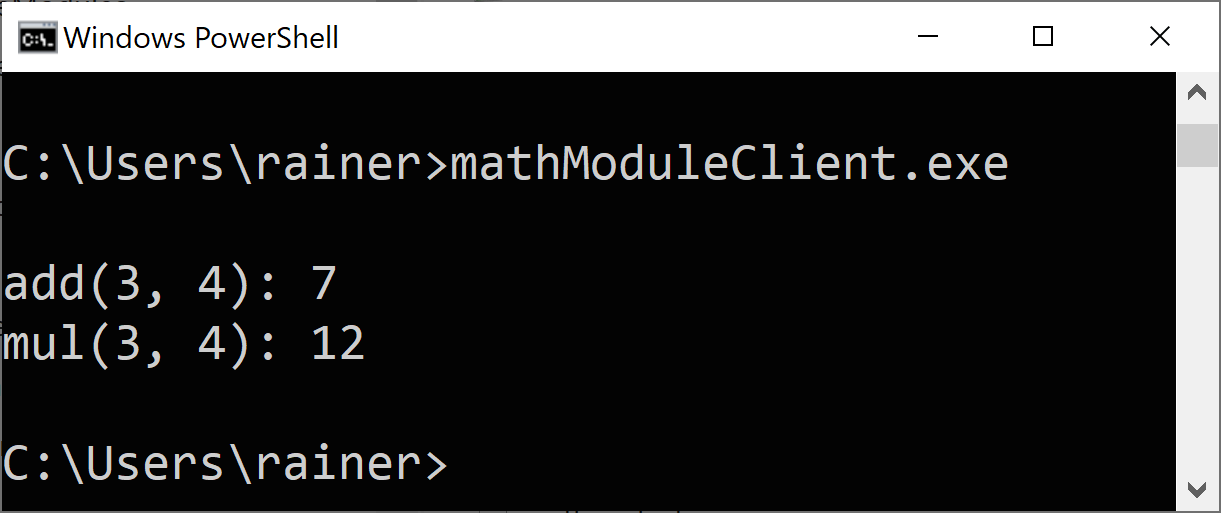
\includegraphics[width=0.6\textwidth]{content/3/chapter4/images/21.png}\\
模块和子模块的用法
\end{center}

\begin{tcolorbox}[breakable,enhanced jigsaw,colback=blue!5!white,colframe=blue!75!black,title={使用Microsoft编译器构建可执行文件}]
	
模块和其子模块一同构建可执行文件

\begin{tcblisting}{commandshell={}}
cl.exe /c /experimental:module mathModule1.ixx /EHsc
cl.exe /c /experimental:module mathModule2.ixx /EHsc
cl.exe /c /experimental:module mathModule.ixx /EHsc
cl.exe /EHsc /experimental:module mathModuleClient.cpp \
  mathModule1.obj mathModule2.obj mathModule.obj
\end{tcblisting}

这三个模块的每个编译过程都会创建两个工件:IFC文件(接口文件)*.ifc在最后一行隐式使用,*.obj文件在最后一行显式使用。

\end{tcolorbox}

子模块也是模块,每个子模块都有一个模块声明。用户可以只使用其中之一,所以这里就创建一个只使用math.math1模块的主程序。

\hspace*{\fill} \\ %插入空行
\noindent
主程序只使用子模块math.math1
\begin{lstlisting}[style=styleCXX]
// mathModuleClient1.cpp
#include <iostream>
import math.math1;
int main() {
	std::cout << '\n';
	std::cout << "add(3, 4): " << add(3, 4) << '\n';
}
\end{lstlisting}

\begin{center}
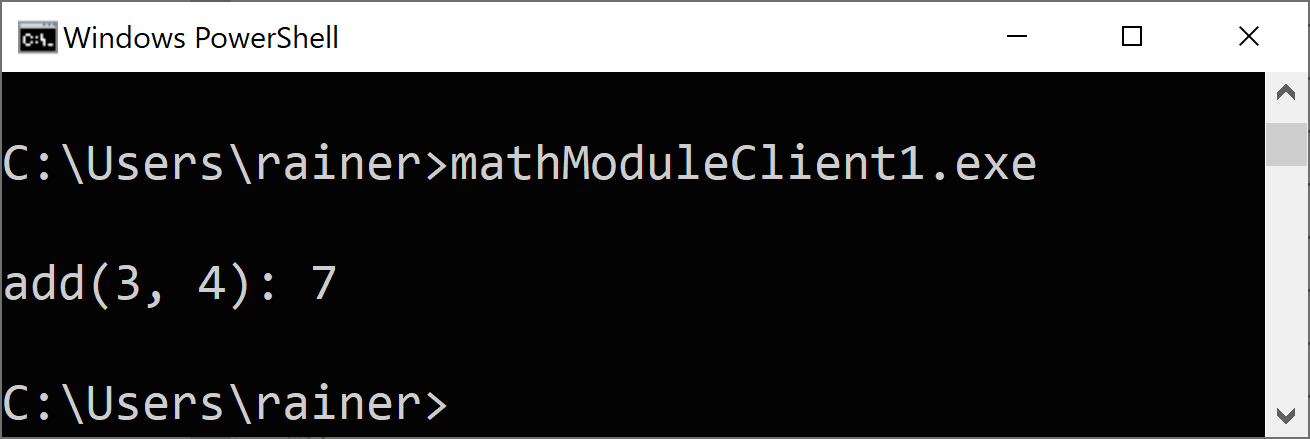
\includegraphics[width=0.6\textwidth]{content/3/chapter4/images/22.png}\\
子模块和模块的用法
\end{center}

将模块划分为模块和子模块,是模块设计者让用户导入部分模块的一种方法,但这个观察结果不适用于模块分区。

\hspace*{\fill} \\ %插入空行
\noindent
\textbf{4.2.8.2\hspace{0.2cm}模块分区}

一个模块可以划分为多个分区。每个分区由一个模块接口单元(分区接口文件)和零个或多个模块实现单元(参见模块接口单元和模块实现单元)组成。分区导出的名称由主模块接口单元(主接口文件)导入和重新导出。分区名称必须以模块名称开头,并且分区不能单独存在。

模块分区的描述比其实现更难理解。下面的代码中,我将为模块分区重写math模块,以及其子模块math.math1和math.math2(参见子模块)。这个过程中,我会介绍模块分区的术语。

\hspace*{\fill} \\ %插入空行
\noindent
\textbf{主接口文件}
\begin{lstlisting}[style=styleCXX]
// mathPartition.ixx

export module math;

export import :math1;
export import :math2;
\end{lstlisting}

主接口文件由模块声明(第3行)组成,使用冒号(第5行和第6行)导入和重新导出分区math1和math2。分区名称必须以模块名称开头,所以不需要指定。

\hspace*{\fill} \\ %插入空行
\noindent
\textbf{第一个模块分区}
\begin{lstlisting}[style=styleCXX]
// mathPartition1.ixx

export module math:math1;

export int add(int fir, int sec) {
	return fir + sec;
}
\end{lstlisting}

\noindent
\textbf{第二个模块分区}
\begin{lstlisting}[style=styleCXX]
// mathPartition2.ixx

export module math:math2;

export {
	int mul(int fir, int sec) {
		return fir * sec;
	}
}
\end{lstlisting}

与模块声明类似,表达式导出模块math:math1和导出模块math:math2(第3行)声明了一个模块接口分区。模块接口分区也是模块接口单元。math代表模块,math1或math2代表分区。

\hspace*{\fill} \\ %插入空行
\noindent
\textbf{导入模块分区}
\begin{lstlisting}[style=styleCXX]
// mathModuleClient.cpp
import math;
int main() {
	std::cout << '\n';
	std::cout << "add(3, 4): " << add(3, 4) << '\n';
	std::cout << "mul(3, 4): " << mul(3, 4) << '\n';
}
\end{lstlisting}

假设用户程序与以前在子模块中使用的程序相同,同样的观察结果也适用于可执行文件的创建和程序的执行:

\begin{center}
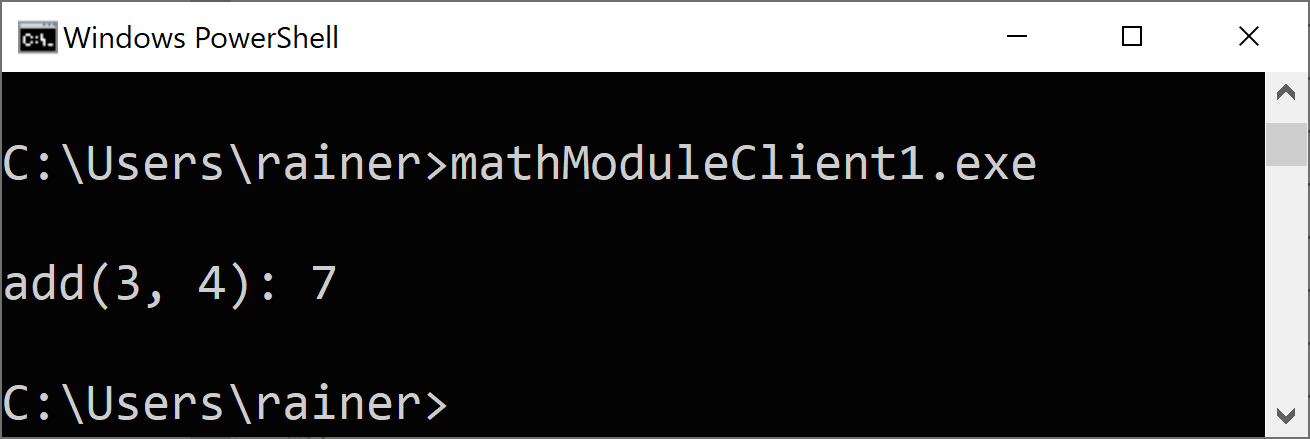
\includegraphics[width=0.6\textwidth]{content/3/chapter4/images/23.png}\\
\end{center}

\subsubsubsection{4.2.9\hspace{0.2cm}模块中的模板}

我经常听到这样的问题:模块如何导出模板?当实例化模板时,其定义必须可用。这就是模板定义放在头文件中的原因。从概念上讲,模板的使用具有以下结构:

\hspace*{\fill} \\ %插入空行
\noindent
\textbf{4.2.9.1\hspace{0.2cm}无模块}

\begin{itemize}
\item 
templateSum.h

\begin{lstlisting}[style=styleCXX]
// templateSum.h
template <typename T, typename T2>
auto sum(T fir, T2 sec) {
	return fir + sec;
}
\end{lstlisting}

\item 
sumMain.cpp

\begin{lstlisting}[style=styleCXX]
// sumMain.cpp
#include <templateSum.h>
int main() {
	sum(1, 1.5);
}
\end{lstlisting}
\end{itemize}

主程序直接包含头文件templateSum.h,sum(1,1.5)触发模板实例化。编译器从函数模板sum中生成具体的函数sum,该函数以int型和double型作为参数。若想要可视化这个过程,请使用\href{https://cppinsights.io/}{C++ Insights}上的示例。

\hspace*{\fill} \\ %插入空行
\noindent
\textbf{4.2.9.2\hspace{0.2cm}有模块}

C++20中,模板应该可以在模块中。模块有一个唯一的内部表示,既不是源代码也不是程序集。这种表示是一种\href{https://en.wikipedia.org/wiki/Abstract_syntax_tree}{抽象语法树}(AST)。由于有了这个AST,模板定义在模板实例化期间可用。

下面的例子中,我在模块math中定义了函数模板sum。

\begin{itemize}
\item 
mathModuleTemplate.ixx

\begin{lstlisting}[style=styleCXX]
// mathModuleTemplate.ixx
export module math;
export namespace math {
	template <typename T, typename T2>
	auto sum(T fir, T2 sec) {
		return fir + sec;
	}
}
\end{lstlisting}

\item 
clientTemplate.cpp

\begin{lstlisting}[style=styleCXX]
// clientTemplate.cpp
#include <iostream>
import math;
int main() {
	std::cout << '\n';
	std::cout << "math::sum(2000, 11): " << math::sum(2000, 11) << '\n';
	std::cout << "math::sum(2013.5, 0.5): " << math::sum(2013.5, 0.5) << '\n';
	std::cout << "math::sum(2017, false): " << math::sum(2017, false) << '\n';
}
\end{lstlisting}
\end{itemize}

编译程序的命令行与前面的没有什么不同,这里直接显示程序的输出:

\begin{center}
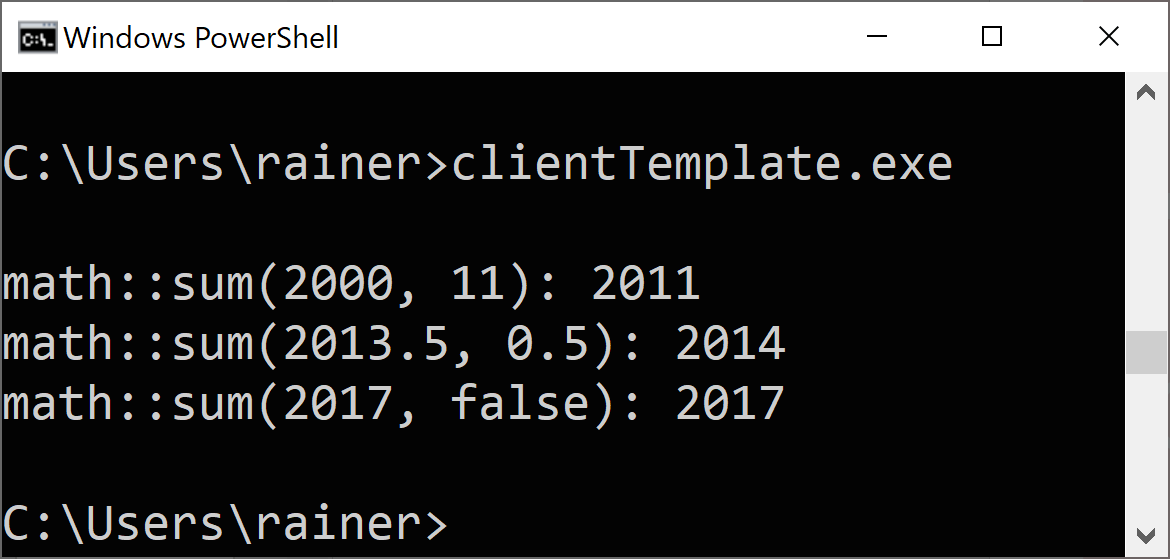
\includegraphics[width=0.6\textwidth]{content/3/chapter4/images/24.png}\\
\end{center}

通过模块,我们得到了一种新的连接方式。

\subsubsubsection{4.2.10\hspace{0.2cm}模块链接}

C++20之前,C++支持两种类型的链接:内部链接和外部链接。

\begin{itemize}
\item 
内部链接:翻译单元之外不能访问具有内部链接,内部链接主要包括声明为静态的命名空间作用域和匿名命名空间的成员。

\item 
外部链接: 具有外部链接的名称可在翻译单元外部访问。外部链接包括声明为非静态的名称、类型及其成员、变量和模板。
\end{itemize}

C++20引入模块连接:

\begin{itemize}
\item 
模块链接: 具有模块链接的名称只能在模块内部访问。若名称没有外部链接且不导出,则视为模块链接。
\end{itemize}

前面的模块声明mathModuleTemplate.ixx的变体说明了这个观点。假设想返回给函数模板sum的用户的不仅是加法的结果,还有编译器推导出的返回类型。

\hspace*{\fill} \\ %插入空行
\noindent
\textbf{改进函数模板sum的定义}
\begin{lstlisting}[style=styleCXX]
// mathModuleTemplate1.ixx

module;

#include <iostream>
#include <typeinfo>
#include <utility>

export module math;

template <typename T>
auto showType(T&& t) {
	return typeid(std::forward<T>(t)).name();
}

export namespace math {

	template <typename T, typename T2>
	auto sum(T fir, T2 sec) {
		auto res = fir + sec;
		return std::make_pair(res, showType(res));
	}

}
\end{lstlisting}

函数模板sum不返回数字的和,而是返回\href{https://en.cppreference.com/w/cpp/utility/pair}{std::pair}(第21行),其中包含sum和res值类型的字符串表示。注意,我将函数模板showType(第11行)放在导出的math命名空间(第16行)之外。因此,不可能在模块math外使用。函数模板showType使用\href{https://www.modernescpp.com/index.php/perfect-forwarding}{完美转发}来保留函数参数t的类型。\href{https://en.cppreference.com/w/cpp/language/typeid}{typeid}运算符在运行时查询有关类型的信息(\href{https://en.cppreference.com/w/cpp/types}{运行时类型标识(RTTI)})。

\hspace*{\fill} \\ %插入空行
\noindent
\textbf{使用改进的函数模板sum}
\begin{lstlisting}[style=styleCXX]
// clientTemplate1.cpp

#include <iostream>
import math;

int main() {
	
	std::cout << '\n';
	
	auto [val, message] = math::sum(2000, 11);
	std::cout << "math::sum(2000, 11): " << val << "; type: " << message << '\n';
	
	auto [val1, message1] = math::sum(2013.5, 0.5);
	std::cout << "math::sum(2013.5, 0.5): " << val1 << "; type: " << message1
			  << '\n';
	auto [val2, message2] = math::sum(2017, false);
	std::cout << "math::sum(2017, false): " << val2 << "; type: " << message2
			  << '\n';

}
\end{lstlisting}

现在,程序显示sum的值和自动推导的类型的字符串表示形式。

\begin{center}
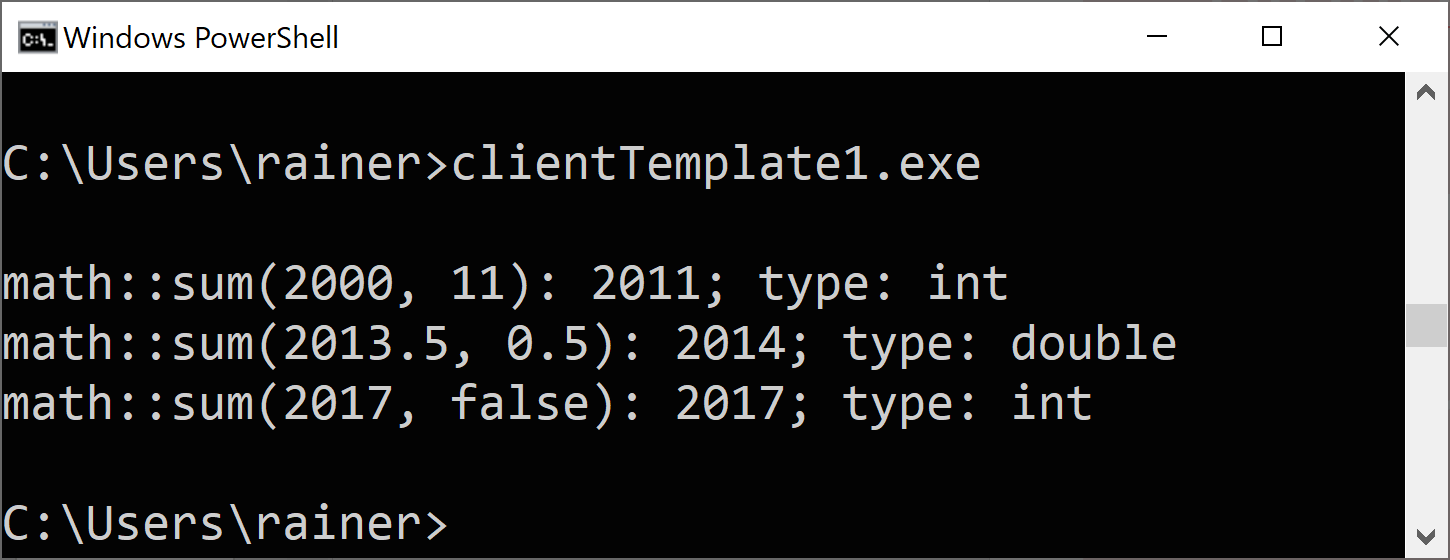
\includegraphics[width=0.8\textwidth]{content/3/chapter4/images/25.png}\\
\end{center}

\subsubsubsection{4.2.11\hspace{0.2cm}头文件单元}

到2020年底,还没有编译器支持头文件单元。头文件单元是一种从头文件转换到模块的平稳方式,只需要用新的import指令替换\#include指令即可。

\hspace*{\fill} \\ %插入空行
\noindent
\textbf{用import指令替换\#include指令}
\begin{lstlisting}[style=styleCXX]
#include <vector> => import <vector>;
#include "myHeader.h" => import "myHeader.h";
\end{lstlisting}

首先,import遵循与include相同的查找规则。所以对于引号("myHeader.h")方式来说,在系统搜索路径之前,会先在本地目录中进行搜索。

其次,这不仅仅是文本替换。编译器会根据import生成类似模块的东西,并将结果视为模块。导入模块语句从头中获取所有可导出的名称,包括宏。导入这些合成的头文件单元比包含头文件要快,并且在速度上与预编译的头文件相当。

\hspace*{\fill} \\ %插入空行
\noindent
\textbf{4.2.11.1\hspace{0.2cm}一个缺点}

头文件单元有一个缺点,并非所有的头文件都是可导入的。哪些头文件可导入\href{https://en.cppreference.com/w/cpp/language/ub}{已经定义好了},但是C++标准保证所有标准库头文件都是可导入的头文件。导入功能排除了C头文件,它们只是简单包装在std名称空间中而已,例如<cstring>是<string.h>的C++包装器。可以很容易地识别包装的C头文件,因为其模式是:xxx.h包装为cxxx。

\begin{tcolorbox}[breakable,enhanced jigsaw,colback=blue!5!white,colframe=blue!75!black,title={使用Microsoft编译器构建可执行文件}]

\begin{itemize}
\item 
模块克服了头文件和宏的缺陷。模块的导入是无开销的,与宏相比,也无所谓导入顺序。此外,还解决了命名冲突。

\item 
模块由模块接口单元和模块实现单元组成。必须有一个模块接口单元,并且具有导出模块声明和任意多个模块实现单元。未在模块接口中导出的名称具有模块链接,不能在模块外部使用。

\item 
模块可以有头文件,也可以导入和重新导出其他模块。

\item 
C++20中的标准库不是模块化的,用C++20构建模块也是一项具有挑战性的任务。

\item 
要构造大型软件系统,模块提供了两种方式:子模块和分区。与分区相反,子模块可以独立存在。

\item 
有了头文件单元,就可以用直接使用import语句替换include,编译器会自动生成一个模块。
\end{itemize}

\end{tcolorbox}

\newpage









































